\documentclass[10pt,twocolumn,letterpaper]{article}
\usepackage[margin=0.75in,columnsep=0.25in]{geometry}
\usepackage[T1]{fontenc}\usepackage[utf8]{inputenc}
\usepackage{mathptmx}\usepackage[protrusion=true,expansion=true]{microtype}
\usepackage{amsmath,amssymb,booktabs,array,tabularx,graphicx,xcolor,enumitem,siunitx,caption,subcaption}
\usepackage{algorithm}\usepackage[noend]{algpseudocode}
\usepackage[numbers,sort&compress]{natbib}
\usepackage[colorlinks,linkcolor=blue!50!black,citecolor=blue!50!black,urlcolor=blue!50!black]{hyperref}
\usepackage[capitalise,noabbrev]{cleveref}
\usepackage[most]{tcolorbox}
\usetikzlibrary{positioning}
% Shared notation. One definition per symbol; sections must not redefine.
\newcommand{\EZ}{EurekaZero}
\newcommand{\searchone}{search\,$=$\,1}
\newcommand{\TBD}[1]{\textcolor{red}{\textbf{[TBD:~#1]}}}
\newcommand{\writer}{\pi_{\theta}}
\newcommand{\referee}{\mathcal{R}}
\newcommand{\inc}[1]{\mathrm{inc}(#1)}
\newcommand{\encP}{\phi_{\mathrm{P}}}
\newcommand{\encS}{\phi_{\mathrm{S}}}
\newcommand{\reward}{r}
\newcommand{\mapv}{v}
\newcommand{\Prob}{\mathcal{P}}
\newcommand{\opp}{\mathcal{O}}
\newcommand{\Sol}{\mathcal{S}}
\renewcommand{\Game}{\mathcal{G}}
\newcommand{\Cwin}{C_{\mathrm{win}}}
\newcommand{\Cattempt}{C_{\mathrm{attempt}}}
\newtcolorbox{keyidea}{colback=blue!4,colframe=blue!40!black,boxrule=0.4pt,arc=1pt,left=4pt,right=4pt,title=Key idea,fonttitle=\bfseries\small}
\newtcolorbox{explainer}[1]{colback=gray!5,colframe=gray!50!black,boxrule=0.4pt,arc=1pt,left=4pt,right=4pt,title={#1},fonttitle=\bfseries\small}
% Missing figure files render as a labelled placeholder instead of failing.
\let\EZincludegraphics\includegraphics
\renewcommand{\includegraphics}[2][]{\IfFileExists{#2}{\EZincludegraphics[#1]{#2}}{\fbox{\parbox[c][1.2in][c]{0.9\linewidth}{\centering\small\textcolor{red}{Figure pending: \texttt{\detokenize{#2}}}}}}}

\hypersetup{
  pdftitle={EurekaZero: Engineered Intelligence for Algorithm Invention by Self-Play},
  pdfauthor={JopeDime Team},
  pdfsubject={Learning to propose algorithms from referee feedback},
  pdfkeywords={algorithm discovery, self-play, expert iteration, program synthesis, single-proposal evaluation}}
\title{{\huge\bfseries \EZ{}}\\[6pt]
  {\Large Engineered Intelligence for Algorithm Invention by Self-Play}}
\author{JopeDime Team}
% A fixed date keeps rebuilds of the committed PDF reproducible.
\date{Draft --- October 2026}
\begin{document}
\maketitle
\begin{abstract}
Can experience from algorithm discovery improve the first proposal for a
new problem? We frame invention as a game in which an encoded task is the
board, an executable program is the move, a verifier supplies feedback and
an incumbent defines improvement. \EZ{} aims to retain that feedback in a
program writer, so deployment can use one complete candidate without
retries or reranking. We separate this proposal budget from the costs of
encoding, generation and fitting, and distinguish measured training behavior
from the stronger claim of transfer to unseen problems. The available
training record does not establish a single-proposal advantage. We specify
comparisons against frontier-designed algorithms, a tabular foundation
model and agents allowed repeated attempts, together with a test of the
problem--program map. \TBD{Complete the independent evaluations, identify
the evaluated checkpoint and replace this draft statement with supported
results and uncertainty.}
\end{abstract}

% ===========================================================================
% Section 1 -- Introduction: Can Machines Invent?
% File: sections/01_introduction.tex
% Reader question: Can an AI create knowledge no human wrote down?
% One-sentence answer: Skeptics say models trained on history can only
%   recombine it. AlphaGo Zero showed that a learner with a referee can go
%   beyond history, and we test that for invention.
% Core points advanced: 4 (skeptics right about imitation, wrong about
%   learning), 3 (search = 1), 1 (innovation is a game).
% Exhibits: Figure 1 (front matter, label fig:emptysquare) and Box 1.
% Budget: 1.5 pages. Editor notes: sections/01_introduction.notes.md
% ===========================================================================

\section{Can Machines Invent?}\label{sec:intro}

Can a machine create knowledge that no human has written down? The strongest
skeptics say no: a model trained on the record of human knowledge can only
recombine it. Go suggests another answer. AlphaGo Zero, taught by a referee
instead of a record, went beyond the best human play without seeing a human
game \citep{silver2017mastering}. We ask whether a similar training signal
can improve algorithm invention: can learning from past evaluations make
the first proposal on a new problem more useful?

\paragraph{The skeptics' challenge.}
In March 2025, Yann LeCun argued that language models retrieve existing
solutions rather than find new ones: ``in their purest form, they are incapable
of inventing new things'' \citep{lecun2025bigtech}. The same month, Thomas Wolf
warned that current trends will give us ``a country of yes-men on servers''
\citep{wolf2025einstein}. Dwarkesh Patel had asked Dario Amodei in August 2023
what to make of models with ``basically the entire corpus of human knowledge
memorized'' that had not made ``a single new connection that has led to a
discovery'' \citep{patel2023question}. In January 2025, Demis Hassabis posed
the hardest version as a benchmark for general intelligence: today's systems
``can play a game of Go at a world champion level. But could a system invent
Go?'' \citep{hassabis2025bigtech}. These challenges separate producing an
unfamiliar idea from learning which ideas will work. Predicting historical
text does not directly reward improvement over an incumbent. That motivates
a different training signal; it does not establish a ceiling on what a
pretrained model can discover (\cref{sec:anatomy}).

\paragraph{Humans are bounded by history too.}
Research effort keeps rising while its productivity
falls: Moore's law now needs more than 18 times as many researchers as in the early 1970s \citep{bloom2020ideas}. Under a growing burden
of knowledge, inventors reach the frontier later and specialize more narrowly
\citep{jones2009burden}. Papers and patents have grown less likely to
break with the past \citep{park2023disruptive}, and fields open to outsiders
when their leading scientists die \citep{azoulay2019funeral}. The bottleneck is
not a shortage of minds. It is the gravity of what we already know.

\paragraph{From search to learning.}
Automated research systems already couple proposals to tests. The AI
Scientist \citep{lu2024aiscientist} and the AI co-scientist
\citep{gottweis2025coscientist} run agentic research loops; AlphaEvolve evolves
programs against automated evaluators \citep{novikov2025alphaevolve}; and
Karpathy's autoresearch retains training changes that improve a measured
objective \citep{karpathy2026autoresearch}. Socher's \emph{Eureka Machine}
extends this vision to agents working with simulators and autonomous
laboratories \citep{socher2026bookbite,socher2026eureka}. These systems make
judgment executable. Our question is what their evaluations can teach the
system that proposes the next idea. Keeping a winning program preserves an
output; training a proposer on those outcomes may preserve a capability that
transfers to a new problem.

\begin{keyidea}
Can judgment bought during training improve the first proposal at deployment?
\end{keyidea}

\paragraph{The Zero move.}
Go faced the same choice and took the other road. AlphaGo learned from human
expert games and searched heavily at every move \citep{silver2016mastering}.
AlphaGo Zero learned only from games against itself, and its network alone,
with no search, rated 3,055 Elo. That is close to the 3,144 of AlphaGo Fan, the
version that beat the European champion Fan Hui
\citep{silver2016mastering,silver2017mastering}. This motivates an analogous
goal for invention: learn from repeated program evaluations during training,
then deploy a writer with a single candidate budget, \searchone{}
(\hyperref[box:searchone]{Box~1}). The budget is a test condition, not a
promise that every first proposal wins. \Cref{fig:emptysquare} summarizes
the distinction between spending search at deployment and learning from it
in advance.

\begin{explainer}{Box 1: What ``search = 1'' means}
\phantomsection\label{box:searchone}%
\begin{itemize}[leftmargin=*,nosep]
  \item \textbf{One inference, one candidate.} For a new problem, the program
    writer emits one complete program ($B = 1$), with no retries, repairs,
    best-of-$N$, reranking or weight updates.
  \item \textbf{Everything is counted,} including reasoning tokens and problem
    encoding. One inference is one generation, not one forward pass.
  \item \textbf{Declare the fitting procedure.} Fitting the emitted algorithm
    to training rows is allowed. Any internal model or hyperparameter
    selection must be disclosed and counted in its compute budget. One
    outer proposal does not establish the absence of internal search.
    Training search is priced separately in \cref{sec:price}.
\end{itemize}
\textbf{A single candidate, with prior knowledge:} the writer starts from
pretraining and human ideas. The Zero analogy concerns the training signal;
it does not imply that the system starts without human knowledge.
\end{explainer}

\begin{figure}[t]
  \centering
  \fbox{\parbox{0.88\linewidth}{\TBD{Conceptual diagram: distinguish search
  during training from the candidate budget at deployment.}}}
  \caption{\textbf{Learning before deployment and searching during it.}
  A conceptual comparison is pending; no measured \EZ{} advantage is implied.}
  \label{fig:emptysquare}
\end{figure}

\paragraph{The proposal and its test.}
We formulate algorithm invention as a game: the encoded problem is the board,
a complete program is the move, a verifier is the referee and the incumbent
algorithm is the opponent (\cref{sec:game}). \EZ{} combines a program writer
with a problem--program map intended to guide learning from those contests
(\cref{sec:method}). The central hypothesis is that this training improves
first proposals on unseen problems. The current learning record is reported
separately from the proposed deployment comparisons.

\Cref{sec:results} specifies the evidence needed to test that hypothesis:
paired comparisons against algorithms proposed by Claude, Codex and Gemini;
a comparison with KumoRFM \citep{kumorfm2025}; a performance curve against
agents allowed repeated attempts; and an ablation of the problem--program
map. \TBD{Complete these comparisons and document task coverage, model
versions, prompts, budgets and uncertainty before claiming an advantage.}
The paper develops five elements:
\begin{enumerate}[leftmargin=*,nosep,label=\arabic*.]
  \item \textbf{The anatomy of innovation:} four pillars (aim, variation,
    judgment and retention), with an idealized relation between proposal
    quality and the number of attempts (\cref{sec:anatomy}).
  \item \textbf{The innovation game:} rules that make invention playable on
    many boards (\cref{sec:game}).
  \item \textbf{The economics of algorithmic self-play:} an accounting of
    training cost and the cost per verified improvement (\cref{sec:price}).
  \item \textbf{\EZ{}:} a writer and a problem--program map designed to learn
    from referee feedback (\cref{sec:method}).
  \item \textbf{An evaluation plan:} tests of first-proposal quality,
    deployment search and the map's contribution (\cref{sec:results}).
\end{enumerate}
\Cref{sec:road} traces each pillar's history in AI; \cref{sec:meaning} asks
what changes and where the claim stops.

To see what the referee can teach, we first separate the parts of innovation.

\section{The Anatomy of Innovation}\label{sec:anatomy}
% Reader question: What is innovation made of?
% Core points advanced: 2 (novelty is free; judgment is the inventor) and
% 4 (right about imitation, wrong about learning); sets up 1 (innovation is a game)
% and 3 (search = 1).
% Table 1 is defined at the start of the section so that the full-width
% float can reach the top of the page where Section 2.2 discusses it.
\begin{table*}[t]
  \caption{\textbf{A four-part reading of traditions of discovery.} A dash marks a pillar outside a tradition's scope: Wallas analyzed a single act of thought. For Darwin and Campbell, the aim is a criterion set by the environment. Engineering is the design--build--test--learn cycle \citep{nielsen2016engineering}; AlphaGo Zero follows \citet{silver2017mastering}; \EZ{} is defined in \cref{sec:game,sec:method}.}
  \label{tab:pillars}
  \centering
  \small
  \setlength{\tabcolsep}{4pt}
  \begin{tabular}{@{}>{\raggedright\arraybackslash}p{0.17\linewidth}>{\raggedright\arraybackslash}p{0.19\linewidth}>{\raggedright\arraybackslash}p{0.19\linewidth}>{\raggedright\arraybackslash}p{0.17\linewidth}>{\raggedright\arraybackslash}p{0.2\linewidth}@{}}
    \toprule
    Tradition & Aim & Variation & Judgment & Retention \\
    \midrule
    \citet{darwin1859origin} & Fitness to the environment & Variation & Natural selection & Inheritance \\
    \citet{wallas1926art} & Preparation & Incubation, illumination & Verification & --- \\
    \citet{campbell1960bvsr} & A selection criterion & Blind variation & Selection & Retention \\
    \citet{popper1963conjectures} & The problem & Conjecture & Refutation & The surviving theory \\
    The scientific method & Question & Hypothesis & Experiment & Publication \\
    Engineering & Design target & Design and build & Test & Learn \\
    AlphaGo Zero & Win the game & Moves chosen with search & Game outcome & Network weights \\
    \midrule
    \EZ{} & Problem encoding and metric & Program writer & Referee on hidden folds & Incumbent pool and weights \\
    \bottomrule
  \end{tabular}
\end{table*}

We organize innovation into four roles: aim, variation, judgment and
retention. They connect a proposed program to its evaluation and to what
the next attempt can learn. We call judgment learned before the next attempt
\emph{taste}, and ask whether it can improve the first proposal.

\subsection{Novelty is free}\label{sub:anatomy-novelty}

Novelty is the cheapest part of invention. Borges imagined a library of every possible book of 410 pages \citep{borges1941babel}. Every algorithm short enough to fit in a volume is already on its shelves. Nothing in the library tells a reader which volume is true. A random string generator is the same library with a faster librarian: almost every string it emits is new, and almost none is worth running (\cref{fig:novelty-judgment}, lower right).

\begin{figure}[t]
  \centering
  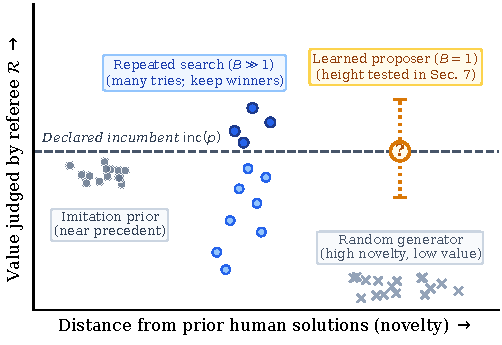
\includegraphics[width=\linewidth]{figures/fig2_novelty_judgment.pdf}
  \caption{\textbf{Novelty is free; judgment is the inventor.} Schematic. Horizontal: distance from what people have already done. Vertical: value as judged by the referee. A random generator travels far and finds little. Imitation, repeated search and a learned proposer illustrate different ways to select candidates; their positions are conceptual, not measured limits. The value of \EZ{}'s single proposal remains an empirical question for \cref{sec:results}.}
  \label{fig:novelty-judgment}
\end{figure}

Language-model studies test this distinction. In a blinded study with 104 NLP researchers, ideas from a language model were rated more original than experts' ideas ($p < 0.05$) \citep{si2024ideas}. Once 43 experts had spent over 100 hours each carrying out ideas from both pools, the generated ideas lost significantly more ground on every metric \citep{si2025gap}.

Boden had predicted the asymmetry in 1998: machines, she wrote, would find generating new ideas easier than automating their evaluation \citep{boden1998creativity}. These studies motivate a distinction between the novelty of a proposal and
its value after execution; they do not establish that judgment is the only
bottleneck in every domain.

\subsection{The four pillars}\label{sub:anatomy-pillars}

Accounts of discovery from biology, psychology, philosophy and engineering
provide a useful common vocabulary (\cref{tab:pillars}). The four-pillar
organization is our synthesis of these traditions, rather than a claim that
their theories are identical.

\textbf{Aim} fixes the problem and what counts as better. Hamming asked colleagues, ``What are the important problems of your field?'' \citep{hamming1986research}. Pólya's first step is to understand the problem \citep{polya1945solve}, and Popper argued that observation is always selective, so it presupposes a problem \citep{popper1963conjectures}.

\textbf{Variation} proposes candidates. Peirce called abduction ``the only logical operation which introduces any new idea'' \citep[CP~5.171]{peirce1934cp}. Campbell modeled creative thought as blind variation \citep{campbell1960bvsr,simonton2011bvsr}. Koestler located creative acts in bisociation, joining two unrelated frames of thought \citep{koestler1964act}. Boden named three routes to a new idea: combining familiar ideas, exploring a conceptual space and transforming it \citep{boden1998creativity}.

\textbf{Judgment} tests a candidate against something outside the mind that proposed it: the attempted refutation \citep{popper1959logic}, the experiment, peer review, and the referee of the common task framework, which scores every entry on data the competitors never see \citep{donoho2017fifty}.

\textbf{Retention} preserves what survives: inheritance for
\citet{darwin1859origin}, selective retention for
\citet{campbell1960bvsr}, the textbook for a science and the incumbent for a
game. It can store either an output or a way to propose better outputs.
Archiving a winning program does the first; using evaluation feedback to
update the generator attempts the second. This distinction connects the
four pillars to the learning question in \cref{sec:intro}.

Campbell argued that every genuine gain in knowledge needs a mechanism for introducing variation, a consistent selection process, and a mechanism for preserving and reproducing what is selected \citep[p.~381]{campbell1960bvsr}. The aim is what keeps the selection consistent, which makes it the fourth pillar.

\subsection{Taste is judgment moved upstream}\label{sub:anatomy-taste}

Skill in invention is judgment that arrives before the try. For Poincaré, creating meant not making the useless combinations: ``Invention is discernment, choice.'' The sterile combinations, he added, do not even present themselves to the inventor \citep[pp.~324--325]{poincare1910creation}.

Chess masters show the same economy: in de Groot's think-aloud studies they considered about as many moves as weaker players but found the right ones \citep{degroot1965thought}. Chase and Simon studied chunks through perception and recall tasks \citep{chase1973perception}. Much of that knowledge is tacit; experts know more than they can say \citep{polanyi1966tacit}.

AlphaGo's policy network learned to select moves from human expert games,
then refined that judgment through self-play \citep{silver2016mastering}.

Taste has a price we can state. Suppose each try beats the incumbent with a fixed, nonzero probability
$\winprob$, independently of the others. The number of tries up to and including the first win is then geometric, with mean
\begin{equation}
  \mathbb{E}[\Ntries] = \frac{1}{\winprob},
  \label{eq:taste}
\end{equation}
where $\Ntries$ counts all candidate attempts, including incomplete or
invalid outputs and failed executions. Under this fixed-probability,
independent-try model, better proposal quality
shortens the expected search.\footnote{Adaptive search and correlated
proposals need not follow \cref{eq:taste}; independence alone does not say
whether the approximation overstates or understates their cost. Empirical
attempt curves are required for those systems.}

The equation isolates the value of learning before deployment. It does not
rank random generators, pretrained models and agent systems without measuring
their proposal quality. In particular, \searchone{} fixes the number of
candidates a system may submit; it does not require the probability of a win
to approach certainty. A single-candidate system can fail, and every failure
must remain in its reported results. \Cref{sec:price} uses the same idealization
to relate evaluation cost to the cost of a verified improvement.

\begin{keyidea}
Novelty is free. Judgment is the inventor.
\end{keyidea}

\subsection{Learning from a referee}\label{sub:anatomy-history}

People learn much of their taste from the record of their field. Normal science, in Kuhn's account, solves puzzles inside a reigning paradigm \citep{kuhn1962structure}. The record also holds people in place: when a star life scientist dies prematurely, articles by outsiders to the star's collaborators flow into the field, draw on different literature and are disproportionately likely to be highly cited \citep{azoulay2019funeral}.

A model trained to predict text receives a signal about what was written,
rather than a direct score for improving an algorithm. That does not prevent
novel generalization. It motivates supplementing the historical record with
feedback from execution, so a useful departure from precedent can be rewarded.

A referee offers such an additional teacher. AlphaGo Zero learned with no human data, from the rules and the outcomes of its own games, and found strategies outside traditional Go knowledge \citep{silver2017mastering}. Its predecessor had already made such a move. As David Silver told Wired in March 2016, AlphaGo put the chance that a human would play its Move~37 against Lee Sedol at one in ten thousand, and it won that game \citep{metz2016twomoves}.

The knowledge then flowed back to people. In more than 5.8 million moves by professionals from 1950 to 2021, previously unseen moves grew more frequent once superhuman programs arrived, and came with better decisions \citep{shin2023superhuman}. These results establish the possibility in Go. Whether an analogous signal
improves algorithm invention must be measured in the innovation game.

\subsection{Where the pillars live}\label{sub:anatomy-where}

Machines do not remove the pillars; they move them (\cref{tab:where}). The most ambitious swarm design fits the same anatomy. In an October 2026 essay drawn from his book, Socher rests the Eureka Machine on ``a living map of all human knowledge'', ``a unified model of physical reality'', ``high-fidelity digital twins'' and ``fully autonomous physical laboratories'' \citep{socher2026bookbite,socher2026eureka}. On top of them, millions of AI agents critique each other's ideas. In our terms, the map is retention; the model of reality, the twins and the laboratories are faster and better judgment; and the agents supply variation and critique.

Agent search and learning from a referee are complementary. A search can
retain programs, revise its context or update its proposer; calling it a
swarm does not determine which of these it does. The comparison in
\cref{tab:where} therefore isolates a common deployment setting in which
search leaves the proposer's weights fixed. \EZ{} instead aims to use
training evaluations to improve the proposer before a new problem arrives.
Both approaches still need a reliable referee, and the cost of training
must be counted alongside any saving at deployment.

\begin{table}[t]
  \caption{\textbf{Where feedback can be retained.} The agent-search column describes
fixed-weight deployment loops, not every agent system. The \EZ{} column
states the proposed training and deployment protocol. In every column,
people still set the aim.}
  \label{tab:where}
  \centering
  \footnotesize
  \setlength{\tabcolsep}{3.5pt}
  \setlength{\extrarowheight}{2pt}% separates rows whose cells wrap
  \begin{tabular}{@{}>{\raggedright\arraybackslash}p{0.16\linewidth}>{\raggedright\arraybackslash}p{0.21\linewidth}>{\raggedright\arraybackslash}p{0.265\linewidth}>{\raggedright\arraybackslash}p{0.265\linewidth}@{}}
    \toprule
     & Human science & Agent search & \EZ{} \\
    \midrule
    Aim & The researcher chooses & A person writes the goal & Problem encoding and metric, chosen by people for now \\
    Variation & The scientist's ideas & Agents propose and critique & One candidate per test problem \\
    Judgment & Experiments, peer review & Experiments, simulators, autonomous labs & The referee, on hidden folds \\
    Retention & The literature & Logs, archives, a map of knowledge & Incumbent pool and the writer's weights \\
    \addlinespace
    Where taste lives & Years of training, in one head & Weights fixed; context can adapt & Training on referee feedback \\
    Deployment budget & Varies by problem & Multiple adaptive attempts & One candidate; success measured \\
    \bottomrule
  \end{tabular}
\end{table}

The next section traces the methods that connect these four roles.

% =====================================================================
% Section 3 -- The Road to Zero: Five Building Blocks
% File: sections/03_road.tex        Label: sec:road
% Reader's question: What has AI already built for each pillar?
% One-sentence answer: Earlier work supplies the components; the question is
%   whether experience across discovery tasks improves a first complete proposal.
% Core points advanced: 3 (search = 1), 4 (imitation vs. learning),
%   1 (innovation is a game).
% Exhibits: Table 3 (tab:roads), Box 2 (Self-play in 90 seconds).
% Depends on labels: sec:intro, sec:anatomy, eq:taste, sec:game,
%   sec:method, sec:results, sec:meaning, app:history (Appendix A).
% =====================================================================

\section{The Road to Zero: Five Building Blocks}\label{sec:road}

Five lines of AI research connect the four pillars of \cref{sec:anatomy}:
deep learning, program search, reinforcement learning, games and the race
for self-improvement. We trace what each proposes, how it is tested and
what carries forward to the next attempt.\footnote{Each history keeps only the
milestones the argument needs; \cref{app:history} collects the referees
those milestones rely on.}

% ---------------------------------------------------------------------
\subsection{Deep learning gave variation a voice}\label{sub:road-deep}

Deep learning built the variation pillar: machines that propose. Models
learned representations from data \citep{lecun2015deep}. AlexNet
made the case on images \citep{krizhevsky2012imagenet}, the Transformer
modeled sequences with attention \citep{vaswani2017attention}, and empirical
scaling laws related language-model loss to model size, dataset size and
training compute \citep{kaplan2020scaling,hoffmann2022chinchilla}.
\citet{sutton2019bitter} drew the lesson: general methods that use
computation win.

Generative models turned representations into proposals in text, video
\citep{brooks2024sora} and code. Codex solved
28.8\% of the HumanEval programming problems with one sample, and 70.2\%
with 100 samples, counting any that passed the unit tests
\citep{chen2021codex}. That gap illustrates the value of a larger sampling budget. It is not
a direct estimate of the geometric model in \cref{eq:taste}: pass rates
and the probability of beating an incumbent measure different outcomes.

Learned prediction and selection also support scientific discovery:
protein structures that rival experiment in most CASP14 cases
\citep{jumper2021alphafold},
2.2 million crystal structures predicted stable relative to the Materials Project
\citep{merchant2023gnome}, and
halicin, an antibiotic that then treated infections in mice
\citep{stokes2020halicin}.

CLIP put images and captions in one shared space
\citep{radford2021clip}, an analogy for our problem--program ranking map
(\cref{sec:method}).
The reference map learns from programs scored within each problem.
Its ranks can influence search-parent selection
(\cref{sub:method-map}); they neither condition nor screen the writer.
Map-ranking accuracy and first-proposal quality require separate tests.

Representations describe a problem, code generation supplies candidates
and a separate map can rank drafts for search. Executable tests make their
quality observable. \EZ{} proposes training on those outcomes, then
measuring transfer beyond its training tasks.

% ---------------------------------------------------------------------
\subsection{Program search built the variation--judgment loop}\label{sub:road-programs}

Program evolution joined variation to judgment: propose a program, score
it, keep the better ones. \citet{friedberg1958learning} let a machine vary
its own instructions, \citet{holland1975adaptation} made variation and
selection a general method of adaptation, and Lenat's AM and EURISKO
searched concepts and heuristics by measures of interest
\citep{lenat1976am,lenat1983eurisko}. EURISKO takes its name from the Greek
verb behind \emph{eureka}, as ours does. \citet{koza1992genetic} closed the
loop with genetic programming: a population of programs, a fitness function
as referee and selection as coach. Populations retain programs; learned
proposers can also retain patterns for later tasks.

Later work sharpened both halves: superoptimization
\citep{massalin1987superoptimizer}, program synthesis from examples
\citep{gulwani2011flashfill} guided by neural networks
\citep{balog2017deepcoder}, neural architecture search \citep{zoph2017nas},
and AutoML-Zero, which evolved learning algorithms from basic mathematical
operations \citep{real2020automlzero}.

Then language models became the
variation operator. FunSearch found cap-set constructions beyond the best
known \citep{romeraparedes2024funsearch}: verified new solutions within a
fixed task, bought with search. Lion, an optimizer found by program
search, went into production at Google \citep{chen2023lion}. AlphaEvolve
multiplied two $4\times4$ complex matrices with 48 scalar multiplications,
improving on Strassen's algorithm in that setting after 56 years
\citep{novikov2025alphaevolve}. MLEvolve carries the loop into
machine-learning engineering \citep{mlevolve2026}.

\EZ{} adopts executable programs as moves inside this generate--judge loop,
and asks how much of a verified search can transfer into the proposer itself.
DreamCoder already learns reusable libraries and a search-guiding model across
tasks \citep{ellis2021dreamcoder}; a single-candidate evaluation tests how
useful a learned proposal is before additional task-specific search.

% ---------------------------------------------------------------------
\subsection{Reinforcement learning turned retention into taste}\label{sub:road-rl}

Program search retains solutions; policy updates change the proposer.
Reinforcement learning uses the referee's verdicts for those updates.
\citet{bellman1957dp} gave it an equation of value. Samuel's checkers
program improved by playing a copy of itself \citep{samuel1959checkers},
TD-Gammon reached near the best human backgammon players by self-play
\citep{tesauro1995tdgammon}, and DQN learned Atari games from pixels
\citep{mnih2015dqn}. AlphaGo learned from human games and searched at every
move \citep{silver2016mastering}; AlphaGo Zero learned by self-play alone
\citep{silver2017mastering}. AlphaZero mastered three games with one
algorithm \citep{silver2018general}, MuZero learned a model for planning
\citep{schrittwieser2020muzero}, and AlphaStar's league of mutually
exploiting agents reached Grandmaster level in StarCraft~II
\citep{vinyals2019alphastar}.

In expert iteration \citep{anthony2017expert}, search is the teacher and
the network is the student (\cref{box:selfplay}).
Language models also learn from feedback: human preferences
\citep{christiano2017preferences,ouyang2022instructgpt} and rule-based
checks of answers, as in DeepSeek-R1 \citep{guo2025deepseekr1}.

This line of work motivates training on referee-scored play. For \EZ{},
the next step is to define a game whose reward measures relative algorithm
quality, then distinguish gains on training games from transfer to unseen
families.

\begin{figure}[tb]% floats so the text above can fill the column
\begin{explainer}[label=box:selfplay]{Self-play in 90 seconds}
In AlphaGo Zero, a player starts with the rules and plays itself. A short
search before each move finds better moves than instinct would, and the referee
scores each finished game. The network learns to propose the moves the
search chose (its policy) and to predict the winner (its value), so the
next search is stronger. Over millions of games, search is distilled into
intuition \citep{anthony2017expert,silver2017mastering}.
\emph{What if the board were a problem, and the move an invention?}
\end{explainer}
\end{figure}

\begin{table*}[t]
\caption{\textbf{Related approaches retain experience in different forms.}
This qualitative comparison separates output, deployment budget and retained
state. Exact budgets depend on each study's protocol. The last row states
\EZ{}'s design; its proposal quality is still to be tested.}
\label{tab:roads}
\centering
\small
\setlength{\tabcolsep}{4pt}
\setlength{\extrarowheight}{2pt}% separates rows whose cells wrap
\begin{tabularx}{\linewidth}{@{}>{\raggedright\arraybackslash}p{0.2615\linewidth}
                >{\raggedright\arraybackslash}p{0.17\linewidth}
                >{\raggedright\arraybackslash}p{0.155\linewidth}
                >{\raggedright\arraybackslash}p{0.19\linewidth}
                >{\raggedright\arraybackslash}X@{}}
\toprule
System & Output & Deployment budget & Retained experience & Feedback source \\
\midrule
Genetic programming; AutoML-Zero
  & An algorithm & Study-specific search & Selected programs
  & Executable objective \\
AlphaTensor; AlphaDev
  & An algorithm for one family & Task-specific search
  & A policy for that game & Game reward \\
FunSearch; AlphaEvolve
  & An algorithm & Iterative search & Program archive
  & Automated evaluation \\
Research swarms (AI Scientist, autoresearch)
  & Experiments and code & Adaptive attempts & Context, logs and archives
  & Experimental outcomes \\
EvoTune; TTT-Discover; Evolution Fine-Tuning
  & An algorithm or construction & Protocol-specific search
  & Fine-tuned policy or search state
  & Search trajectories \\
TabPFN; MotherNet; KumoRFM
  & Predictions or network weights & Task-specific inference
  & Pretrained parameters & Training across tasks \\
Absolute Zero; STP
  & Answers and proofs & Decoding budget varies & Policy parameters
  & Correctness feedback \\
\midrule
\EZ{}
  & An algorithm & One candidate
  & Proposed writer updates
  & Referee scores ranked within each problem \\
\bottomrule
\end{tabularx}
\end{table*}

% ---------------------------------------------------------------------
\subsection{Gamification made judgment cheap}\label{sub:road-games}

Games built the judgment pillar at scale. \citet{shannon1950chess} chose
chess because its moves and its goal are sharply defined. The common task
framework made machine-learning research a game: shared data, enrolled
competitors and a referee who scores every entry on a sealed test set
\citep{donoho2017fifty}, as in the Netflix Prize \citep{bennett2007netflix}
and ImageNet \citep{russakovsky2015imagenet}. People played science too.
Foldit players beat automated methods on hard protein puzzles
\citep{cooper2010foldit} and solved a protease structure that earlier
attempts had not \citep{khatib2011protease}; EteRNA players, whose designs
were tested in a laboratory, found RNA design rules \citep{lee2014eterna}.

Then machines played problems. AlphaTensor's TensorGame beat the best-known
matrix-multiplication algorithms for several sizes
\citep{fawzi2022alphatensor}, and AlphaDev's AssemblyGame found sorting
routines now in the LLVM C++ library \citep{mankowitz2023alphadev}.
AlphaGeometry learned olympiad geometry without human demonstrations
\citep{trinh2024alphageometry}. AlphaProof, using the Lean proof
checker, and AlphaGeometry~2 jointly reached silver-medal standard on the
2024 International Mathematical Olympiad problems, using computation over
multiple days \citep{hubert2026alphaproof}.

These benchmarks supply the recipe for a game (clear rules, a referee, a
score and a sealed test) and raise the question of which parts of a task can
vary under a shared representation and referee. \EZ{} makes the problem an
input to the proposer (\cref{sec:game}); whether that supports transfer across
families remains a result to establish.

% ---------------------------------------------------------------------
\subsection{The race for self-improvement scaled search}\label{sub:road-self}

The race for self-improvement spans program search, agent scaffolds and learned policies.
\citet{good1966speculations} foresaw an ``intelligence explosion'', and
\citet{schmidhuber2003goedel} specified a G\"odel machine that rewrites its
own code once it proves the rewrite useful.

STOP improves the scaffold that calls a language model, including
itself, and its authors note: ``Since the language models themselves are
not altered, this is not full recursive self-improvement''
\citep{zelikman2024stop}. The Darwin G\"odel Machine's self-editing agents
raised its SWE-bench score from 20.0\% to 50.0\% \citep{zhang2025dgm}, and
AlphaEvolve cut Gemini's training time by 1\%
\citep{novikov2025alphaevolve}.

Language models also play themselves. SPIN plays its previous iteration
\citep{chen2024spin}, Absolute Zero proposes and solves coding tasks under a
code executor \citep{zhao2025absolutezero}, and STP pairs a conjecturer with
a Lean prover \citep{dong2025stp}. \citet{bailey2026sgs} attribute plateaus
in LLM self-play to reward hacking by the conjecturer and evaluate
self-guidance in formal theorem proving. Our closest neighbors learn to
discover. EvoTune
fine-tunes on what its own evolutionary search finds \citep{evotune2025},
and TTT-Discover trains on the one problem at hand, at a few hundred
dollars per problem \citep{tttdiscover2026}. Evolution Fine-Tuning learns
from \num{156000} search trajectories across 371 tasks \citep{eft2026}, and
DiscoRL meta-learned a reinforcement-learning rule that beat human-designed
ones \citep{oh2025discorl}. These approaches retain improvements in different places: a search
trajectory, a task-specific learner or a reusable learning rule. Our
comparison asks about the quality and cost of the first complete candidate,
rather than treating these forms of learning as absent.

Research itself is becoming a swarm. The AI Scientist automates ideas,
experiments and papers \citep{lu2024aiscientist}, and the AI co-scientist
ranks agents' hypotheses in an Elo tournament
\citep{gottweis2025coscientist}. Karpathy's autoresearch, released in March
2026, runs about 100 experiments overnight and keeps what improves
\citep{karpathy2026autoresearch}. In May 2026, Recursive raised
\$650 million to build AI that improves itself
\citep{recursive2026techcrunch}. In the innovation game, an encoded research task would be the board and
its evaluator the referee (\cref{sec:game}).

Self-improvement comes in three strengths: a system can find better external
algorithms, build better components of itself, or improve its own ability to
improve, raising verified discoveries per unit of compute across generations.
Each requires separate evidence (\cref{sec:meaning}); a recorded
training trajectory alone establishes none of them on an unseen task.

These systems motivate two reference requirements: verify an improvement
before retaining it, and sandbox candidate execution
(\cref{sub:method-referee}). The proposed learning test compares a trained
writer with its frozen reference under the same deployment budget;
it is separate from the adapter record in \cref{sec:method-status}.

% ---------------------------------------------------------------------
\subsection{Where the roads meet}\label{sub:road-meet}

\Cref{tab:roads} separates outputs, budgets and retained experience.
The cross-task predictors and network generators
\citep{hollmann2025tabpfn,muller2025mothernet,kumorfm2025} differ from
readable-program output; one candidate does not equalize compute or inputs.
Absolute Zero and STP use correctness feedback. A declared incumbent sets
our comparison standard; \cref{sec:game} defines how the referee judges a
program against it.

\begin{keyidea}
The test is whether experience on earlier discovery tasks improves the first
complete proposal on a new one.
\end{keyidea}

\section{Innovation Is a Game}\label{sec:game}
% Reader question: Can invention be played like Go?
% Core points advanced: 1 (primary: innovation is a game), 2 (novelty is free;
% judgment is the inventor), 3 (search = 1)
% Exhibits: Table 4 (tab:go-vs-innovation), Figure 3 (fig:game-loop)

We define one attempt at algorithm invention as a game: the encoded
problem is the board, a program is the move, the referee checks and
scores it, and a declared incumbent is the opponent.

Encoding the problem
provides a shared interface; each task type still needs its own qualified
encoding, language and evaluation protocol (\cref{sub:game-boards}).


% ----------------------------------------------------------------------------
\subsection{Why games came first}\label{sub:game-games}

Games became AI's laboratory because they supply four things at once: fixed
rules, an impartial referee, a clear winner and cheap replay. Chess was chosen
because it is ``sharply defined both in allowed operations (the moves) and in
the ultimate goal (checkmate)'' \citep{shannon1950chess}, and checkers showed
that a program could improve by playing itself \citep{samuel1959checkers}.

Together these properties support repeated, reproducible evaluation. People
scale judgment the same way, through prizes, leaderboards and the common task
framework's ``scoring referee'' \citep{donoho2017fifty} (\cref{sec:road}).
Invention has the first three properties once the problem and the solution are
written down, within the limits of \cref{sub:game-played}; cheap replay is a
question of cost (\cref{sec:price}).

% ----------------------------------------------------------------------------
\subsection{The rules}\label{sub:game-rules}

\Cref{tab:go-vs-innovation} sets the game beside Go. An illegal move is
counted as a failed attempt. The reference writer reads the encoded problem.
The referee keeps the incumbent as a separate comparison standard
(\cref{sub:method-board}); its code and score must stay outside the writer's
input.

\begin{table}[!htb]
  \caption{\textbf{Go and the innovation game, element by element.}
  Moves differ most: Go's are cheap, while each program is costly to judge
  (\cref{sub:game-played}). Go's game length is
  from \citet{silver2016mastering}.}
  \label{tab:go-vs-innovation}
  \centering
  \small
  \setlength{\tabcolsep}{4pt}
  \setlength{\extrarowheight}{2pt}% separates rows whose cells wrap
  \begin{tabular}{@{}>{\raggedright\arraybackslash}p{0.18\linewidth}>{\raggedright\arraybackslash}p{0.32\linewidth}>{\raggedright\arraybackslash}p{0.42\linewidth}@{}}
    \toprule
                   & Go                              & The innovation game \\
    \midrule
    Board          & Stones on a $19\times19$ grid   & The encoded problem \\
    Move           & Place one stone, or pass        & Write one complete program \\
    Legal move     & Empty point; no suicide or forbidden repetition & Parses, type-checks, runs within limits \\
    Illegal move   & Not allowed                     & Stillborn: an automatic loss \\
    Referee        & The rules of Go                 & The verifier, on hidden folds \\
    Win            & Higher final score             & Valid, and beats the incumbent \\
    Opponent       & A past self                     & The incumbent, often a past self \\
    Rating         & Elo                             & Win rate and Elo across problems \\
    Moves per game & About 150, each cheap           & One, costly to judge \\
    \bottomrule
  \end{tabular}
\end{table}
% Figure 3 is defined here, ahead of its first reference, so that the
% full-width float can reach the top of the page where it is cited.
\begin{figure*}[t]
  \centering
  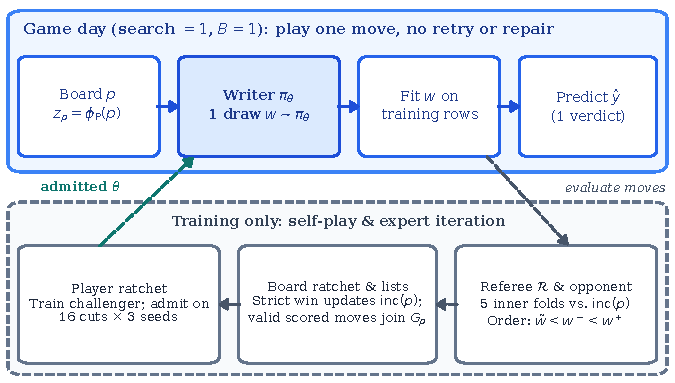
\includegraphics[width=\textwidth]{figures/fig3_game_loop.pdf}
  \caption{\textbf{Training plays the whole game; game day plays one move.}
  Schematic. Top row (blue): game day. Dashed box: training only. Outcomes
  are recorded; valid scored programs can enter the learning lists, while
  failed attempts still count against the budget.}
  \label{fig:game-loop}
\end{figure*}

Formally, the game is a tuple of seven parts,
\[
  \Game = (\Prob, \encP, \Sol, \encS, \referee, \reward, \opp).
\]
Here $\encP$ and $\encS$ embed a problem $p \in \Prob$ and a program
$w \in \Sol$ as $z_p$ and $z_w$. The referee $\referee$ reports a program's
validity and score, the reward $\reward$ orders moves, and the opponent $\opp$
supplies the incumbent $\inc{p}$. The tuple extends Rice's model of algorithm
selection \citep{rice1976algorithm}: the player writes the algorithm instead of
picking it, and a declared incumbent sets the comparison standard.

With one move, the game is a contextual bandit: the board supplies context,
the program is the action and the
verdict is the reward \citep{lattimore2020bandit}. It earns the name through an
opponent that improves as the player does. The asymmetry is in the
moves: Go offers about 250 legal moves per turn over about 150 turns, each free
to check \citep{silver2016mastering}, while this game offers one move, costly to
judge. Under a single-attempt budget, the chance $\winprob$ of a win matters
directly (\cref{eq:taste}). Whether training raises that chance on new
families is the test in \cref{sec:results}.

\Cref{fig:game-loop} draws the loop. Game day plays only its top row, so
nothing can send a move back for another try; that is \searchone.

% ----------------------------------------------------------------------------
\subsection{The board and the move}\label{sub:game-board}

The board is the aim pillar of \cref{sec:anatomy}, made machine-readable: a
summary of the training data, the objective and metric, and the constraints.
Landmark scores from cheap learners \citep{pfahringer2000landmarking} and
learned tabular summaries are possible encodings. The reference checkpoint
in \cref{sub:method-board} uses a frozen 2,048-value summary with a
30-second cap.
A useful board should preserve distinctions relevant to algorithm choice,
remain stable under irrelevant reorderings, exclude final evaluation
information and have a measured cost. These are requirements to test, not
properties guaranteed by naming an encoder. People still choose the problem
and define what counts as a useful solution.

A move is one program in a typed language over learning primitives.
The reference language uses a 401-token
vocabulary, with up to six transforms chosen from 31 and one of 22 prediction
heads (\cref{sub:method-move}).

Types remove whole classes of stillborn
programs before they run \citep{montana1995stgp}. Canonicalization can merge
syntactic variants; it need not identify every functionally equivalent
implementation. AutoML-Zero
reused scores when hashes of truncated predictions matched after a short
training and validation probe \citep{real2020automlzero}. Matching a probe
does not establish agreement on other inputs (\cref{sub:method-move}).

The language bounds what can be expressed; changing its primitives changes
that space \citep{boden1990creative}. The reference grammar also bounds
composition depth. Structural constraints can prevent invalid programs; their effect on useful proposal
quality must be measured (\cref{sec:results}).

% ----------------------------------------------------------------------------
\subsection{The referee and the opponent}\label{sub:game-referee}

The reward is an ordering first and a number second. Validity is a gate: any
stillborn program scores below any valid one. Past the gate, programs rank by
improvement over the incumbent on hidden folds. The reference promotion
rule keeps the existing incumbent on a tie. Novelty never pays for losing: any novelty
bonus (\cref{sec:price}) must respect the order. For a stillborn program
$\tilde{w}$, an also-ran $w^-$ and a win $w^+$ on board $p$,
\[
  \reward(p, \tilde{w}) \;<\; \reward(p, w^-) \;<\; \reward(p, w^+).
\]

The opponent is a ratcheting incumbent. In the reference procedure, only
strict improvement on five inner folds under the same evaluation protocol
can displace a board's incumbent.
A retrained writer has a separate
admission test on 16 held-out cuts with three seeds each
(\cref{sub:method-selfplay}). Together the two ratchets make this self-play:
the player keeps facing a standard often set by its own earlier play.
AlphaGo Zero likewise separated network admission from choosing a move
during play \citep{silver2017mastering}.

Subtracting the incumbent's score does not change which move is best.
Promotion raises the bar, turns yesterday's winners
into today's also-rans and shifts which problems are worth playing. The
reference learning targets use each program's rank within its scored list
(\cref{sub:method-map,sub:method-selfplay}).

% ----------------------------------------------------------------------------
\subsection{One game, many boards}\label{sub:game-boards}

Binary and multiclass classification, regression, ranking, forecasting and
relational prediction are prospective boards. A shared formal interface
still needs a compatible encoding, program language, metric and validation
protocol qualified for each task type.

Beyond machine learning, examples of referees include sorting tests
\citep{mankowitz2023alphadev}, evaluators for mathematical constructions
\citep{romeraparedes2024funsearch} and accelerator-kernel timers
\citep{novikov2025alphaevolve}. These motivate extensions of the recipe,
rather than results of this paper (\cref{sec:meaning}).

Casting algorithm discovery as a game is not new, but earlier games wrote one
family of problems into their rules, as AlphaTensor did for matrix
multiplication and AlphaDev for sorting
\citep{fawzi2022alphatensor,mankowitz2023alphadev}. AlphaZero used one algorithm
for three games and trained a separate network for each
\citep{silver2018general}. Here the problem is an input on the board, so one
player can, in principle, learn many boards.

\begin{keyidea}
A reliable referee makes a discipline a candidate for this game; transfer
to that discipline still needs evidence.
\end{keyidea}

% ----------------------------------------------------------------------------
\subsection{The analogy's limits}\label{sub:game-played}

A worked game, chosen by a rule fixed before inspection, is to be reported with
the results (\cref{sub:results-failures}). The analogy breaks in four places.

\textbf{The referee is noisy}: picking a
winner by a noisy validation score biases that score upward
\citep{cawley2010overfitting}. Strict numerical improvement alone does not
quantify confidence; independent evaluation and an uncertainty protocol are
needed to interpret it.

\textbf{Moves are expensive}, each a fit and a cross-validation
(\cref{sec:price}).

\textbf{Judges can be gamed}, as METR documented for
frontier models in June 2025 \citep{metr2025rewardhacking}; \cref{sec:method}
lists our safeguards.

And \textbf{no algorithm wins everywhere}: averaged
uniformly over all problems, no learner has lower error off the training set
than another, ours included \citep{wolpert1996nfl}.

Real problems are structured, though, and a player that
reads the board can choose its bias board by board. \Cref{sec:results} reserves the tests of that hypothesis against fixed
frontier-designed algorithms, with paired outcomes beside Elo summaries
\citep{elo1978rating}. Non-transitive comparisons are one reason not to
reduce the evidence to a single rating \citep{balduzzi2018reevaluating}.

Those rules define an attempt. Pricing a verified improvement must also
count attempts that fail or lose.

% =====================================================================
%  EurekaZero -- Section 5: The Price of Play
%  File: sections/05_price.tex   (compiles under the shared preamble)
% =====================================================================
\section{The Price of Play}\label{sec:price}
% Reader question: Can anyone afford to play it?
% One-sentence answer: Yes; cost per win is cost per attempt divided by the
%   win rate, so wasted moves set the bill, not token prices.
% Core points advanced: 3 (search = 1) and 2 (search length is the
%   reciprocal of taste); supports 1 (cheap replay is what invention lacks).
% Exhibits: Equation 2 (eq:bill), Table 5 (tab:price), Figure 4 (fig:price), Box 3.
% Numerical scenarios are retained from the supplied Section 5 source drafts.
% A reproducible calculation artifact remains pending.

What would it cost to play the innovation game? Under the planning
assumptions below, generation and updates for a 30B-class open-weight writer
cost about \$12,000 in GPU time. This is a partial compute projection, not
an observed price for a complete training run. Encoding, input tokens,
repairs and referee execution must be added to the ledger. Cheap
replay is the one property of Go that invention lacks (\cref{sec:game}). Here
we separate planning assumptions from the measurements still required in
\cref{sec:results}.

\subsection{The bill in one line}\label{sub:price-bill}

For repeated attempts with a fixed win probability, expected cost per win
is mean cost per attempt, repairs included, divided by that probability:
\begin{equation}
  C_{\text{win}} = \frac{C_{\text{attempt}} + \mathbb{E}[r]\,C_{\text{repair}}}{q}.
  \label{eq:bill}
\end{equation}
Here $C_{\text{attempt}}$ is the cost of one try, including the referee's
fit; $C_{\text{repair}}$ is the cost of one repair turn, and $\mathbb{E}[r]$
the mean number of repairs per attempt. The $q$ is that of \cref{eq:taste},
the probability that one try beats the incumbent: what sets the number of
tries also sets the price. It factors as $q = q_{\text{run}}\,q_{\text{beat}}$,
the share of moves that run times the share of those that win. A move that
runs and loses still costs money, so we divide by $q$, not by the survival
rate. Generating a token costs about 2~FLOPs per active parameter, and
training on one about~6 \citep{kaplan2020scaling}. We give self-hosted
projections and dated API-price examples (\cref{sub:price-run}).

The bill has two ledgers. Training pays for every attempted candidate,
including failures; deployment pays for encoding, one proposal and its
fitting procedure, with no repair. Fixed-weight agent loops instead buy
evaluation during task-specific search; a trained proposer may amortize
some of that work across later tasks. Whether the saving repays training
requires a measured crossover, still pending in \cref{sec:results}.

\subsection{Wasted moves}\label{sub:price-waste}

An attempt can fail before or after it becomes a valid competitor.
A stillborn move never competes: it fails
to parse or type-check, crashes, times out or returns degenerate output. An
also-ran runs and loses. The planned funnel in \cref{fig:price}a traces
those stages and the compute spent before each failed attempt stops. If 90\% of attempts fail to improve the incumbent, the independent-try
model requires ten attempts per improvement in expectation. A typed program language
removes many stillborn moves by construction (\cref{sec:game}), and those
that remain usually fail before the costly fit. Whether also-rans dominate is a pilot question. Learning, a changed search
procedure or a changed opponent can affect the measured win rate; isolate
the effect attributed to the writer.

\begin{figure}[t]
  \centering
  \includegraphics[width=\linewidth]{figures/fig4_price.pdf}
  \caption{\textbf{Pilot cost measurements pending.} Planned panels:
  (a)~the share of development proposals that run, score, beat the incumbent
  and survive re-verification, with the compute spent at each stage;
  (b)~cost per verified win by writer size and reasoning effort.
  \TBD{Supply pilot data, seeds and family-level uncertainty; identify
  settings with no verified win without assigning a finite cost per win.}}
  \label{fig:price}
\end{figure}

\subsection{The correction tax and the reasoning dial}\label{sub:price-tax}

Small models are cheap per token and can be dear per win. Compute per token
falls about 190-fold from a dense 1.5T writer to an 8B one, so the small
model is cheaper per win unless its win rate per attempt is more than 190
times lower, repairs counted. That threshold flatters the small model:
repair turns re-read a growing context, and a writer that needs three times
the tokens per attempt breaks even at about 60, not 190.

Reasoning is the second dial. Reasoning tokens may cut stillborn moves, but
each is billed as output. \Cref{fig:price}b maps cost per win over writer
size and reasoning effort. A U-shaped curve is the hypothesis; the
measurement decides where, and whether, the minimum sits.

\subsection{Rewarding useful hallucination}\label{sub:price-hallucination}

A pretrained writer pulls toward the textbook answer, which is history's
taste. On a board whose incumbent is that answer, it is an also-ran by
definition. A \emph{useful hallucination} is a move the pretrained prior rates
unlikely and the referee confirms (Box~3). Four counterweights push the
writer toward such moves: a novelty bonus paid only inside the validity gate
(\cref{sec:game}), temperature and entropy schedules, a curriculum that
starts past known solutions, and a quality-diversity archive
\citep{lehman2011novelty,mouret2015mapelites}. \Cref{sec:method} states which
of these \EZ{} uses. Novelty also raises waste, so exploration gets a stated
share of games, \TBD{X\%}.

\begin{explainer}{Box 3: Why a referee makes hallucination safe}
  \label{box:hallucination}
  In text, a hallucination is an error nobody checks. In a game, an
  unfamiliar move is a conjecture, and the referee checks every one.
  Unfamiliar and verified is a discovery; unfamiliar and unchecked is
  confabulation. In March 2016, AlphaGo's own estimate put the chance that a
  human would play its Move~37 against Lee Sedol at about one in ten
  thousand \citep{metz2016twomoves}, and AlphaGo won the game. A referee does
  not make strange moves good. It makes them cheap to try, and it is only as
  trustworthy as what it measures (\cref{sec:method}).
\end{explainer}

\subsection{How many games?}\label{sub:price-games}

Three quantities differ by orders of magnitude.
\textbf{Tries to find one improvement:} $1/q$ on average (\cref{eq:taste}).
If tries were independent, $q = 1\%$ would need 69 tries for even odds and
299 for 95\% confidence; tries from one writer are correlated, so these are
guides, not guarantees.
\textbf{Experience to train a transferable player:} AlphaGo Zero generated
4.9 million self-play games in about three days \citep{silver2017mastering},
and AlphaZero played 44 million games of chess in about nine hours
\citep{silver2017chess,silver2018general}. Our planning budget of 10,000
problems, 100 rounds and 8 attempts gives 8 million attempts, the same order.
It counts work, not learning: problem families matter more, and pilot
learning curves decide, read only within their measured range.
\textbf{Precision to plan the test:} illustratively, 150 independent
units at a win rate near 60\% give an approximate 95\% interval of
$\pm 8$ points. The actual study must compute uncertainty over independent
families, rather than treating every dataset as an independent observation.

\subsection{A run, priced}\label{sub:price-run}

\Cref{tab:price} prices an 8-million-attempt run for six writers: about
\$12,000 with a 30B-class writer and about \$570,000 with a dense 1.5T one.
The dense 1.5T rollouts take $1.2\times10^{23}$~FLOPs, about 1\% of a $10^{25}$-FLOP
pretraining run, a scale more than 30 public models had reached by mid-2025
\citep{rahman2025over30,epoch2024data}. Mixture-of-experts (MoE) writers pay
compute on their active parameters, such as the 32B of 1T in Kimi~K2 \citep{kimiteam2025k2}
or the 37B of 671B in DeepSeek-V3 \citep{deepseekv3}. They need memory for
all of them: 1T one-byte weights fill at least 13 H100s.

\begin{table}[t]
  \centering
  \caption{\textbf{Projected generation and update costs for a fixed
  attempt budget.} These totals exclude other components of a full run;
  the number of verified wins remains to be measured. Projections before pilots; [low-cost, high-cost] in
  brackets. Base: 8 million attempts of 5,000 generated tokens; \$2.92 per
  H100-hour on 29 October 2026 \citep{ornn2026ocpi} [\$2.50, \$4.17;
  \citealp{thunder2026gpu}]; 989.5 dense BF16 TFLOP/s per GPU
  \citep{nvidia2026h100}; generation at 20\% of peak [30\%, 10\%], or 10\%
  [20\%, 7\%] for memory-bound mixture-of-experts (MoE) writers; updates on
  10\% of tokens at 40\% of peak [50\%, 30\%]. The 1.5T rows are scenarios.
  Excludes input tokens, repairs and the referee. \$k: thousands of dollars;
  assumptions and numerical scenarios from the supplied cost drafts.
  \TBD{Supply a reproducible calculation artifact before publication.}}
  \label{tab:price}
  \small
  \begin{tabular}{@{}l l S[table-format=2.2] S[table-format=2.2] l l@{}}
    \toprule
    Program writer & {Active} & {GPU-h per} & {\$ per} & {Rollouts, 8M} & {Updates,} \\
                   & {params} & {1,000 attempts} & {1,000 attempts} & {attempts (\$k)} & {full run (\$k)} \\
    \midrule
    Small dense & 8B & 0.11 & 0.33 & 2.6 [1.5, 7.5] & 0.4 [0.3, 0.7] \\
    Mid dense & 32B & 0.45 & 1.31 & 10.5 [6.0, 30.0] & 1.6 [1.1, 3.0] \\
    Large dense & 70B & 0.98 & 2.87 & 23.0 [13.1, 65.6] & 3.4 [2.4, 6.6] \\
    1T MoE & 32B & 0.90 & 2.62 & 21.0 [9.0, 42.8] & 1.6 [1.1, 3.0] \\
    1.5T MoE (scenario) & 50B & 1.40 & 4.10 & 32.8 [14.0, 66.9] & 2.5 [1.7, 4.7] \\
    1.5T dense (scenario) & 1.5T & 21.05 & 61 & 492 [281, 1405] & 73.8 [50.5, 140] \\
    \bottomrule
  \end{tabular}
\end{table}

The referee runs on CPUs, at 10 to 100 CPU-seconds per move and
\$0.015--\$0.045 per vCPU-hour \citep{doit2026c7i}. For a full run that is
\$330--\$990 at 10 seconds and \$3,300--\$9,900 at 100, enough to exceed an
8B writer's whole bill. List prices sit above our floor. On 30 October 2026,
Together AI listed \$0.60 per million output tokens for gpt-oss-120B (5.1B
active) and \$0.14 for an 8B Llama model
\citep{together2026pricing,openai2025gptoss}: about 7 and 2 times our floor
for the same model. The running example's single game cost \TBD{\$c}:
\TBD{t} generated tokens and \TBD{s} CPU-seconds of referee time.

\begin{keyidea}
  Cost per verified improvement depends on both the cost of an attempt
  and the probability that it wins.
\end{keyidea}

The table prices a fixed number of attempts, not a fixed number of wins.
Converting those totals to cost per win requires a measured win rate. Under
\cref{eq:bill}'s fixed-probability accounting, doubling $q$ halves the
expected cost per win while leaving the per-attempt bill unchanged.

The scaling scenarios in this section concern 8B--1.5T language-model
writers producing 5,000 tokens per attempt; they do not price the reference
checkpoint in \cref{sec:method}. That checkpoint uses a compact network with 27.8 million parameters and at most 128 grammar-constrained tokens, with no repair
in the proposed single-candidate deployment protocol. Its measured costs
must be reported separately from the scaling projections.

The method's job is to improve proposal quality; whether it does so must be
measured under the stated deployment budget.

% sections/06_method.tex — Section 6, EurekaZero: Learning Taste
% Reader question: How does a model learn taste?
% Core points advanced: 3 (search = 1) and 4 (learning from referee feedback); supports 1.
% Historical reference specifications come from the supplied source notes.
% Checkpoint acceptance and reference runtime receipts remain required.
% Historical source notes are archived outside the paper tree.
\section{EurekaZero: Learning Taste}\label{sec:method}

The reference architecture for tabular regression pairs a program writer
with a separate ranking map. Verified search supplies their training
targets; the proposed deployment protocol asks for one new program.
We describe that reference first, then distinguish the later
adapter-ranking record in \cref{sec:method-status}.

\subsection{The player in one picture}\label{sub:method-picture}

\Cref{fig:network} connects training to the single-candidate contract in
\cref{box:searchone}. A frozen encoder reads the board and the program
writer $\writer$ writes one complete program, as AlphaGo's policy
network proposed a move \citep{silver2016mastering}. The problem--program map
$\mapv$ supplies a separate ranking score. In the native implementation it
neither conditions nor screens the writer. The proposed game-day protocol
omits it, permitting only the writer's single draw under \searchone{}.

\begin{figure*}[t]
  \centering
  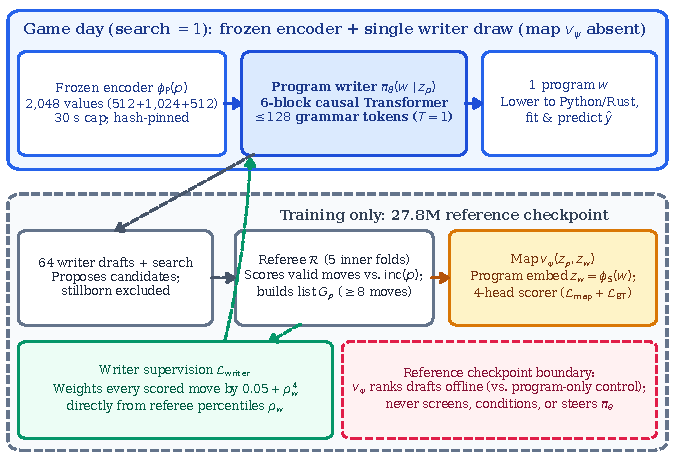
\includegraphics[width=\textwidth]{figures/fig5_network.pdf}
  \caption{\textbf{A writer and a separate ranking map learn from scored programs.} Historical reference schematic. Top:
  game day, the whole of \searchone{}. Dashed box: training only. Search seeded with the writer's
  drafts proposes more programs, the referee scores them against the incumbent, and the scored
  lists retrain the writer ($\theta$) and the map ($\psi$). Stillborn programs enter no list.}
  \label{fig:network}
\end{figure*}

\subsection{Reading the board}\label{sub:method-board}

The reference regression encoder turns the board of \cref{sec:game}
into 2,048 numbers, $z_p=\encP(p)$, in three blocks.
The first summarizes a pretrained row encoder's embeddings across rows,
independent of row order (512 values). The second projects the hidden
state of a pretrained third-party tabular regressor that reads the training
rows and labels (1,024; third-party provenance pending; restricted; redistribution prohibited). The third passes the
scaled targets through two frozen windows (512).

The reference encoder is pinned by hash and stays fixed during writer
training. Encoding is bounded at 30 seconds per problem. A context with any non-finite value is refused
rather than imputed (\cref{app:training}). The input contract permits
training-side task evidence only; final held-out labels and their derived
statistics must stay outside the input closure. A context's recorded
declaration that no final target was used establishes neither input closure
nor numerical qualification. CPU contexts require native replay and bounded-execution receipts before accepted-policy use.

Whether problems with similar best programs sit together requires a
separate representation study; \cref{sub:results-ablation} reserves that test.

\subsection{Describing the move}\label{sub:method-move}

A move is one program in the typed language of \cref{sec:game}, with a
401-token training inventory listing 31 transforms and 22 prediction heads; the product runtime restricts executable heads.
The writer emits a flat operator-and-slot token stream with a fixed
beginning, engine and regression-task header, rather than parenthesis
tokens or the \texttt{pipe} wrapper. Its nine-phase grammar mask permits
up to six transform stages and three expression stages; each expression
tree is bounded at depth four and 15 nodes
\citep{kusner2017grammar,dai2018sdvae}. After the end token, detokenization
renders a parenthesized program that must parse before entering the pool.
The mask has no remaining-token-budget check: a draw without an end token
at the 128-token horizon, including the fixed header, is incomplete and
discarded. Grammar legality does not establish successful execution or
useful quality. The proposal
pool removes exact decoded-string duplicates and records their SHA-256.
The executor also records canonical recipe hashes. Probe-based behavior
matching is a separate audit, not part of pool deduplication. Without probe
evidence, this behavior check reports novelty as unknown. Readable Python
and Rust exports are a reference requirement. Legacy recipe emitters reject
the synthesized input stage; the separate fitted-state path is allowlisted.
Reported winners still require the parity check in \cref{sub:method-referee}.

\subsection{One map for problems and programs}\label{sub:method-map}

The map reads a program as $z_w=\encS(w)$, the layer-normalized mean of
non-padding token embeddings, including \texttt{BOS}, the fixed engine and
task header, and \texttt{EOS}. Pooling discards token order, limiting its
ability to distinguish compositions built from the same tokens.

The map's own two-layer context network projects the 2,048-value $z_p$
to $r_z\in\mathbb{R}^{512}$. It joins three 512-value blocks: $z_w$
as is, $z_w\odot\tanh(W_\gamma r_z+b_\gamma)$, and
$|z_w-(W_{\mathrm{proj}}r_z+b_{\mathrm{proj}})|$.
Four two-layer heads receive this same 1,536-value interaction vector;
their mean gives $\mapv(z_p,z_w)$ with parameters $\psi$.
Native ranking losses supervise that mean jointly, without separate
targets or bootstrap samples. Training applies dropout of 0.05 in each
ranking head. The runtime head instead reads $[r_z,z_w]$, while the
program-only control reads $z_w$.

Higher logits rank higher within a problem. The score is not a calibrated
error estimate. Comparing its magnitude across problems or reading it as a
probability of a verified win requires separate evidence. The referee
still establishes validity and measures performance.

The map learns from scored lists. For each problem $p$ with at least eight
scored programs, $G_p$ holds them and $\rho_w\in[0,1]$ is a program's
percentile, 1 for the best. The map's softmax over the list is trained toward a target concentrated on the best
\citep{cao2007listnet}:
\begin{equation}
  \mathcal{L}_{\text{map}}(p)=-\sum_{w\in G_p}
  \frac{e^{\rho_w/\tau}}{\sum_{u\in G_p}e^{\rho_u/\tau}}\,
  \log\frac{e^{\mapv(z_p,z_w)}}{\sum_{u\in G_p}e^{\mapv(z_p,z_u)}},
  \label{eq:mapLoss}
\end{equation}
with $\tau=0.25$. With a unique best program, the low-temperature limit
concentrates the target on that program. This is a listwise ranking
objective over programs scored on the same problem; the analogy to
contrastive learning \citep{oord2018cpc,radford2021clip} does not establish
CLIP-style alignment across problems and programs.
A Bradley--Terry term adds pairwise comparisons on the same lists
\citep{bradley1952rank}. Stillborn moves have no score, so this ranking
objective covers only programs that run.

A program-only head trained beside it provides a control for testing
whether the map uses problem context (\cref{sec:results}).

\begin{keyidea}
The reference game-day protocol omits the ranking map. Its single proposal
tests what the writer has learned.
\end{keyidea}

In the native implementation, the writer and map use separate context
networks and token embeddings. The map ranks the draft pool without
dropping drafts or screening the writer.

One native GP route weights
seeded-survivor parent selection by map rank. The bounded search driver
instead cycles among up to four parents selected by measured loss. The map's
influence on training therefore depends on the search route.

Only the 64 neural or fallback seeds receive normalized rank weights;
the 16 tail seeds enter unscored. Unscored survivors share the lowest
scored survivor weight while scored survivors remain.

Native assembly reserves ten tail slots for cut teachers or fallbacks
and six for random exploration. Teacher-first execution prioritizes
retained cut teachers. The reference layout is in \cref{alg:selfplay}.

The writer's loss weights programs by referee rank. Ranking agreement with the referee
and program-only control assesses ranking; better proposals require a
matched ablation (\cref{sub:results-ablation}).

\subsection{The self-play loop}\label{sub:method-selfplay}
% Algorithm 1 is defined at the start of the subsection so that the full-width
% float can reach the top of the next page.
\begin{algorithm*}[t]
\caption{The reference self-play loop (training).}\label{alg:selfplay}
\begin{algorithmic}[1]
\Require training problems; serving writer $\writer$ and map $\mapv$; incumbents $\inc{p}$
\For{each round}
  \For{each sampled training problem $p$}
    \State $z_p \gets \encP(p)$; keep the first 64 distinct valid draws from $\writer(\cdot\mid z_p)$ \Comment{$T=1$; grammar-uniform fill if short}
    \State verified search, seeded with the drafts and 16 random exploration programs, proposes more programs \Comment{the teacher}
    \State $\referee$ fits and scores each distinct program on 5 inner folds \Comment{stillborn: no score}
    \State \textbf{if} a program strictly beats $\inc{p}$ \textbf{then} it becomes $\inc{p}$ \Comment{board ratchet}
    \State add every scored program to the list $G_p$ \Comment{winners and also-rans}
  \EndFor
  \State train a challenger $(\theta',\psi')$ on the lists
  \State \textbf{if} it beats $\writer$ on held-out cuts \textbf{then} $(\theta,\psi)\gets(\theta',\psi')$ \Comment{player ratchet}
\EndFor
\end{algorithmic}
\end{algorithm*}

The historical reference uses expert iteration \citep{anthony2017expert}:
verified search supplies the writer's training programs. Programs sampled
from the scored lists $G_p$ are weighted by referee rank in the combined
objective (\cref{app:training}):
\begin{align}
  \mathcal{L}_{\text{writer}}(p) &= -\sum_{w\in G_p}\bigl(0.05+\rho_w^{4}\bigr)\log\writer(w\mid z_p),
  \label{eq:writerLoss}\\
  \mathcal{L} &= \mathcal{L}_{\text{writer}} + 0.1\,\mathcal{L}_{\text{map}}
  + 0.25\,\mathcal{L}_{\text{BT}} \nonumber\\
  &\quad + 0.1\,\mathcal{L}_{\text{runtime}} + 0.05\,\mathcal{L}_{\text{prog}}.
  \label{eq:totalLoss}
\end{align}
The writer loss in \cref{eq:writerLoss} is schematic: it displays the rank
weights. The native implementation also smooths grammar-legal targets,
averages token losses within each program, and normalizes by the sum of
program weights (\cref{app:training}).

Here $\mathcal{L}_{\text{BT}}$ is a Bradley--Terry loss on the same lists,
$\mathcal{L}_{\text{runtime}}$ a Huber loss between $\ln(1+s)$ and
$\ln(1+\operatorname{softplus}(h))$, where $s$ is nonnegative measured
seconds and $h$ is the raw runtime-head output, and
$\mathcal{L}_{\text{prog}}$ the Bradley--Terry loss of the program-only control head.
A median-ranked program carries about a tenth of the top-ranked program's
weight in the writer loss. Its referee score also contributes to the map's
ranking targets.

The reference procedure uses two ratchets (\cref{sec:game}). A program
displaces a board's incumbent only by strictly beating it.

Under the reference admission rule, a retrained writer faces 16 cuts with
three seeds each. It replaces the serving writer
only if its mean log error ratio favors it. It must also win at least as
many cuts as it loses and fail no more often.
%
Here a cut is a held-out evaluation case fixed before the admission test.
For each cut, the rule takes the natural log of paired best-error ratios
(challenger divided by serving) and averages over matched seeds; it then
averages across cuts. Negative values favor the challenger. This admission
comparison is separate from the single-program comparison in
\cref{sub:results-learning}.

\paragraph{The historical reference.} The writer is a decoder-only transformer (six blocks, width 512)
that reads the context as a prefix token and writes at most 128 tokens; with the map, the network
has 27.8 million parameters. The supplied source notes describe training on eight A100 GPUs in
September 2026, with a corpus of about 10.2 million scored programs from
80 training datasets. \Cref{alg:selfplay,app:training} give the reference
specifications.

These specifications do not supply the checkpoint's acceptance evidence or
qualify its runtime. Both records remain inputs to the evaluation contract
(\cref{sub:results-protocol}). The accepted native checkpoint route is
limited to tabular regression, and the native training entry point remains
held at its grant gate. Numerical parity of the CPU float32 Candle port
with the native CUDA BF16 tch runtime remains unqualified; random streams
and uniform-token fallback differ.

\subsection{Keeping the referee honest}\label{sub:method-referee}

Search supplies training targets only as reliably as its referee.
A learner rewarded by a referee can exploit its flaws. In February 2025 Sakana AI walked back
claims after its AI CUDA Engineer exploited the evaluation code \citep{sakana2025walkback}. In June
2025 METR reported frontier models patching their scorers \citep{metr2025rewardhacking}, and 16\% of
1,968 agent-benchmark tasks can be passed without being solved \citep{zhong2026hackerfixer}.

The evaluation protocol must withstand such attacks. Selection,
promotion and final scoring must use separate data (inner folds, held-out
cuts, a final fold scored once), with sealed meta-test families outside the
learner's inputs.

The proposed comparisons require sandboxed execution
using seccomp and Landlock, with memory, swap and time limits. A
planted label leak and a sealed canary must both be caught. Every reported
winner must be re-run from its emitted code, with native and emitted
predictions agreeing within
$10^{-9}\max(1,|\hat y|)$.

One earlier leaderboard entry for our search selected each dataset's best
test-scored outcome from a ledger of 63,108 evaluations; we exclude it as test selection (\cref{app:incidents}).

\subsection{Game day: \texorpdfstring{\searchone}{search = 1}}\label{sub:method-gameday}

\begin{algorithm}[tb]
\caption{Proposed game-day protocol (\searchone).}\label{alg:gameday}
\begin{algorithmic}[1]
\Require new regression problem $p$ with training rows and metric; frozen $\encP$ and $\writer$
\State $z_p \gets \encP(p)$ \Comment{read the board}
\State $w \sim \writer(\cdot \mid z_p)$, one draw at $T=1$ \Comment{one move; no retry}
\State $f \gets \textsc{Fit}(w,\ \text{training rows})$ \Comment{as any algorithm is fit}
\State $\hat{y} \gets f(\text{new rows})$ \Comment{a stillborn $w$ scores as a loss}
\State \Return $w,\ \hat{y}$
\end{algorithmic}
\end{algorithm}

\Cref{alg:gameday} instantiates the contract in \cref{box:searchone} for
regression, with a recorded seed and frozen components. That contract
fixes the candidate budget, failure handling and full cost boundary.

Report later search
separately, as \citet{silver2017mastering} reported
AlphaGo Zero's raw network apart from its search (\cref{sec:results}).

The deployment budget is a protocol constraint; improvement in the first
proposal requires the matched comparison in \cref{sub:results-learning}.
The development record in \cref{sec:method-status} concerns an adapter that
ranks a pool, a different task from proposing a new program.
% Auto-included at the end of Section 6. Every number below is read from
% figures/data/*.csv (derived by figures/scripts/extract_flywheel.py).
\subsection{Where training stands}\label{sec:method-status}
We report the live training loop as it is, not as we hope it will be.
\Cref{fig:fw-validation} shows every candidate the adapter proposed over
695 consecutive rounds (rounds 775--1469). Only 4 were admitted; the best
validation utility, 1.1378, has not been exceeded since. \Cref{fig:fw-trainval}
shows the reason we treat this as a plateau rather than a pause: on every
logged round, training utility sits 0.282--0.290 above validation utility, a
generalization gap that further adapter steps have not closed. The frozen
encoder's checksum matched on every round; only the adapter trains.
\Cref{fig:fw-telemetry} gives the loop's operating envelope.

\begin{figure}[t]
  \centering
  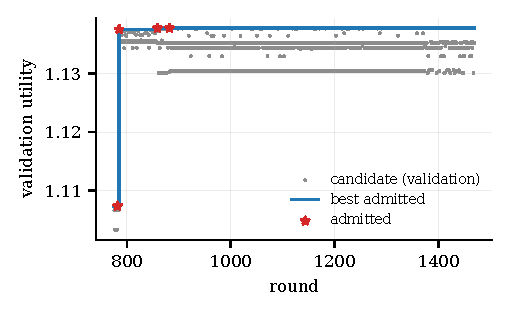
\includegraphics[width=\linewidth]{figures/fig_fw_validation.pdf}
  \caption{\textbf{Validation utility has plateaued.} Grey: each round's
  candidate adapter on the validation families. Blue: best admitted model.
  Stars: the four admitted candidates (rounds 775--1469).}
  \label{fig:fw-validation}
\end{figure}

\begin{figure}[t]
  \centering
  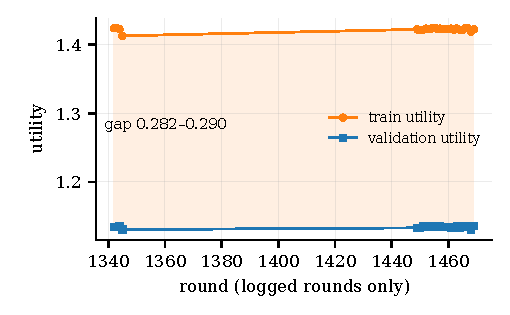
\includegraphics[width=\linewidth]{figures/fig_fw_train_val.pdf}
  \caption{\textbf{Train and validation utility, with the gap shown.} Only
  rounds whose full summaries are retained are plotted (25 rounds between
  1342 and 1469); the line joins non-consecutive rounds across the gap.}
  \label{fig:fw-trainval}
\end{figure}

\begin{figure*}[t]
  \centering
  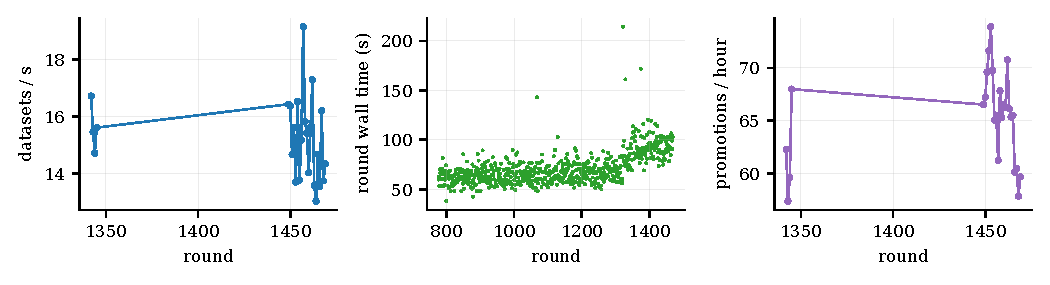
\includegraphics[width=\linewidth]{figures/fig_fw_telemetry.pdf}
  \caption{\textbf{Loop telemetry.} Left: datasets evaluated per second.
  Middle: wall time between consecutive rounds. Right: programs promoted into
  the pools per hour. The run directory occupied 290\,MB at the snapshot.}
  \label{fig:fw-telemetry}
\end{figure*}


\section{Results}\label{sec:results}

Does training make the first proposed algorithm better on an unseen problem?
The available training trajectory in \cref{sec:method-status} records
validation behavior during learning. It does not answer the deployment
question: those validation outcomes inform admission and are not an
untouched test. This section specifies the comparisons still needed.
\TBD{Add independent evaluation evidence before making a performance claim.}
\TBD{Supply a source-bound benchmark before claiming deployment throughput.}

\paragraph{Earlier search diagnostics.}
The supplied method notes report 3,227 exact ties in 3,268 paired
policy-seeded versus generic final searches, plus a separate audit in which
98.84\% of reported winners were already in their starting seed populations.
The paired searches shared seeds, repeated development contexts and had
unequal wall times; they were not independent first-proposal draws. The two
historical inventories differ.

For a separate earlier model evaluated on development contexts, the notes
report fresh-program pairwise ranking accuracy of 0.506 with an interval
of [0.441, 0.568], which includes chance. The reference checkpoint and later adapter snapshot in
\cref{sec:method} require their own ranking evidence.
These observations describe historical search and ranking behavior; the
matched first-proposal test below is still required.
\TBD{Pin the inventories, checkpoints and seeding, timing and ranking
protocols, separately from the final comparisons below.}

\subsection{Evaluation contract}\label{sub:results-protocol}

Freeze the writer, permitted task inputs, output support, decoding rule and
budgets before opening final outcomes. Pin dataset versions and content
hashes, row splits and family assignments. Separate unseen problem
families from training and development, and report which task types were
actually tested.
Report known training and pretraining exposure for the writer, encoders
and learned comparators, with unresolved provenance marked explicitly.
Bound unseen-family claims to the exclusions actually established.
Each \EZ{} submission follows \cref{alg:gameday}; failed generations and
executions remain in the denominator. Report paired results and uncertainty
at the family level, alongside encoding, generation, fitting and prediction
costs. Disclose any internal model or hyperparameter selection in the
emitted procedure, even when the writer submits only one outer candidate.
\TBD{Document the final problem inventory, dataset identities, row splits,
family assignments and exclusions, component provenance, evaluator,
checkpoint, seeds, task metrics and failure accounting.}

\subsection{The effect of training}\label{sub:results-learning}

Test the learning claim with a frozen reference writer as the control.
Predeclare that checkpoint and the evaluated training intervention before
opening final outcomes. Hold the encoder, program grammar and output
support, permitted task inputs, decoding rules, fitting protocol, referee
and resource budgets constant; vary the writer checkpoint. Changes to the
support, encoder or evaluator belong in separate conditions.

Pair the first draws under predeclared seeds and report all of them, with
no selection of the best seed or candidate. Report paired family-level
outcomes, failures and costs alongside source-bound evidence of optimizer
updates and parameter changes. \TBD{Supply the matched first-proposal
comparison and training-update evidence before claiming transfer.}

\subsection{One proposal against fixed methods}\label{sub:results-headtohead}

The proposed comparison asks whether one task-conditioned program competes
with methods that run unchanged across tasks. Frontier-designed algorithms
must be fixed before final evaluation; record the originating models,
prompts, dates and implementation checks. Pin the KumoRFM configuration
\citep{kumorfm2025}, disclose its permitted inputs and fitting procedure, and
compare under the same task metrics. \Cref{tab:headtohead} reserves the
comparison; no winner is assumed.

\begin{table}[t]
  \centering
  \caption{\textbf{Planned paired comparisons.} No outcomes are yet supplied.
  Report ties, failures and excluded cases alongside wins.}
  \label{tab:headtohead}
  \small
  \begin{tabularx}{\linewidth}{@{}>{\raggedright\arraybackslash}X>{\raggedright\arraybackslash}X@{}}
    \toprule
    Comparator & Outcome and uncertainty \\
    \midrule
    Claude-designed method & \TBD{paired evaluation} \\
    Codex-designed method & \TBD{paired evaluation} \\
    Gemini-designed method & \TBD{paired evaluation} \\
    KumoRFM & \TBD{paired evaluation} \\
    \bottomrule
  \end{tabularx}
\end{table}

\begin{figure}[t]
  \centering
  \fbox{\parbox{0.88\linewidth}{\TBD{Leaderboard: supply the evaluated methods,
  paired outcomes, rating protocol and uncertainty.}}}
  \caption{\textbf{Leaderboard pending.} Elo is a summary of a specified
  comparison population, not a substitute for paired task results.}
  \label{fig:leaderboard}
\end{figure}

\subsection{The cost of more attempts}\label{sub:results-search}

Compare the single proposal with agents allowed successive attempts and
development feedback. Keep final outcomes unavailable to those agents.
Count every candidate attempt, including incomplete or invalid outputs
and failed executions; a repair that emits a revised candidate is another
attempt. Charge all task-time computation. Plot
performance against both attempts and cost; if an agent does not reach a
reference performance within its budget, report that limit.
\TBD{Supply attempt curves, matched budgets, repeated seeds and uncertainty.}

\begin{figure}[t]
  \centering
  \fbox{\parbox{0.88\linewidth}{\TBD{Search curve: performance versus attempts
  and compute, including failed attempts and unreached targets.}}}
  \caption{\textbf{Deployment search comparison pending.} The single-candidate
  condition fixes a budget; its measured quality remains to be established.}
  \label{fig:searchone}
\end{figure}

\subsection{What the map contributes}\label{sub:results-ablation}

A representation study should test whether nearby problem encodings share
useful programs, with data disjoint from fitting the map. Ranking agreement
should also be compared with the program-only head, so a global preference
for common programs is distinguishable from reading the problem.
\TBD{Supply problem-similarity and program-only-control evaluations.}

A ranking head can agree with a referee without improving the writer.
In the checkpoint described in \cref{sub:method-map}, the map neither
conditions nor screens the writer's draw. Its ranking accuracy therefore
cannot establish a reduction in wasted proposals. A causal ablation needs
a declared route by which the map changes training, with the writer,
training budget and deployment protocol otherwise matched.
\TBD{Identify an implemented influence path or limit the study to ranking.}

\begin{table}[t]
  \centering
  \caption{\textbf{Map evidence still required.} Ranking quality and a change
  in first-proposal quality are separate outcomes.}
  \label{tab:ablation}
  \small
  \begin{tabularx}{\linewidth}{@{}>{\raggedright\arraybackslash}X>{\raggedright\arraybackslash}X@{}}
    \toprule
    Question & Required evidence \\
    \midrule
    Does the map rank candidates? & \TBD{held-out ranking study} \\
    Does it improve the writer? & \TBD{matched causal ablation} \\
    Does it reduce execution failures? & \TBD{failure-class comparison} \\
    \bottomrule
  \end{tabularx}
\end{table}

\subsection{Failure cases and a worked example}\label{sub:results-failures}

Describe unsuccessful proposals and coverage limits as well as wins.
Assign each attempt one terminal status: incomplete generation, parse or
type-checking refusal, execution
or resource failure, invalid output under declared checks, and valid ties,
losses and wins. Every attempted candidate contributes its incurred cost.
Unresolved outcomes retain an explicit unknown status; fix their treatment
and the validity rules before opening final outcomes.
\TBD{Supply attempt inventories and costs by outcome class, identifying
unresolved cases.}

Choose the worked example by a rule fixed before inspection, and show its emitted
program, fitting procedure and comparison outcome; if the selected category
is empty, report that fact. \TBD{Supply the example selection rule, actual
program and verified outcomes, with no replacement of failed attempts.}
These results will determine which interpretations in \cref{sec:meaning}
the evidence can support.

\section{Meaning}\label{sec:meaning}

What would a successful single proposal establish, and where would that
claim stop? The answer depends on the independent results in
\cref{sec:results}. The recorded training trajectory alone cannot establish
transfer, useful new composition or autonomous scientific discovery.
\TBD{Reconcile every conclusion below with the completed evaluation.}

\subsection{Learning to select and learning to invent}

A better task-dependent choice from a fixed program archive demonstrates
selection. A useful composition absent from the training archive is a stronger
result, and requires an output space that permits it. Token-by-token decoding does not distinguish the two:
report the admissible output space, the training archive and the relation
of each proposed program to that archive. \TBD{State which claim the evaluated
checkpoint and its outputs actually support.}

\subsection{Moving judgment across problems}

If learning improves first proposals on new families, it would support the
hypothesis that training evaluations can be retained as a transferable
proposal capability. It would not show that one proposal wins on every
problem. Test-time search may still improve a learned writer, and its value
should be compared with the training cost it takes to improve that writer.
\TBD{Use the measured search curves and full cost account to bound this claim.}

\subsection{The referee defines the boundary}

The framework optimizes what its referee measures. Repeated development
comparisons can overfit that referee, while a restricted language can hide
useful algorithms from the learner. Task representations, training families
and runtime limits further bound the result. A referee for a new scientific
domain would need its own validity and cost evidence; analogy to a game
supplies neither. \TBD{Report observed failures, distribution shifts and
remaining tests of the referee.}

\subsection{A bounded claim about self-improvement}

Improving an external algorithm, improving the proposer and improving the
rate at which the proposer learns are distinct claims. Evidence for the
first does not establish the others. People still choose the task, metric,
representation and resource limits. \TBD{State the strongest supported level
of improvement and leave untested extensions as future work.}

The contribution to assess is concrete: whether retained evaluation
experience improves the first executable proposal on a new problem, under
a declared budget and an independently scored test.

\appendix
\section{Historical notes}\label{app:history}\TBD{appendix content}
\section{Incident log}\label{app:incidents}\TBD{appendix content}
\section{Training details}\label{app:training}\TBD{appendix content}

\bibliographystyle{plainnat}
\bibliography{refs}
\end{document}
